
 \section{Regularization}
\textbf{Bias of method M}: \\
distance of average model $\bar{f} = \frac{1}{K}\sum_{k=1}^{K}\hat{f}_k$ to the ground truth $f^{*}(x)$: $\mathbb{E}_{x}(f^{*}(x)-\hat{f}(x))^2$ \\
\textbf{Variance of method M}:
average distance of individual models to average model $\mathbb{E}_{x}[\sum_{k=1}^{K}(f^{*}(x)-\hat{f}(x))^2]$ \\
\textbf{Bias variance decomposition and trade-off}: \\
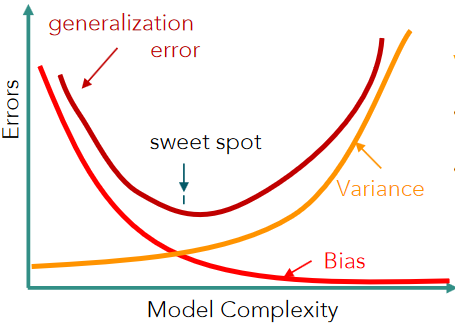
\includegraphics[width=0.35\linewidth]{pics/figure3.PNG} 
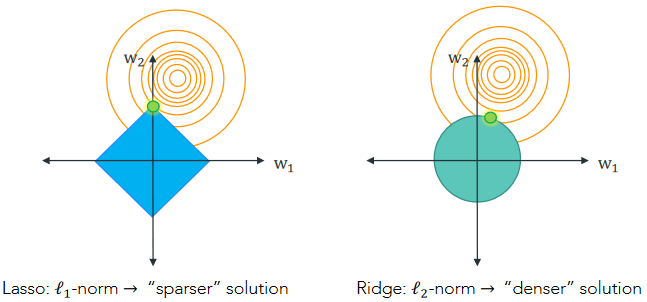
\includegraphics[width=0.6\linewidth]{pics/figure4.PNG}\\
\textbf{Geometric insight of lasso and ridge regression}
\textbf{Model complexity reflected in norms}: \\
- The larger the norm, the larger the space in $\mathbb{R}$ you use $\rightarrow$ higher model complexity \\
- Fitting noise often causes norm/model complexity to increase by using more unnecessary features\\
\textbf{Lasso regression}: (convex)
only use a few of these feature, encourage sparsity via limiting $l_1$-norm. (manually limiting the polynomial degree), \textbf{NO} close form $(\hat{w}^{\lambda}_i) = sign(\hat{w}_i)max(0, |(\hat{w}_i)| - \lambda))$ \\
The problem formulation: $\arg \min_{w}$ $||y - \phi w||^2$ s.t. $||w||_1 \leq R \rightarrow \arg \min_{w}$ $||y - \phi w||^2 + \lambda ||w||_1$\\
\textbf{Ridge regression}
The problem formulation: same as above except $||w||_2^2$ \quad\quad strict convex\\ 

Closed-form solution (find stationary point): $\hat{w_{\lambda}} = (X^TX + \lambda I)^{-1}X^Ty$ (or use the gradient methods) \\

\textbf{Cross-validation for $\lambda$ selection}\\
- Given a choice of features $\lambda$; - Find the best fit model for each fold: $\hat{f}^{\lambda}_k = M_{\lambda}(D_k) = \arg \min_{f} L_0(f;D_k) + \lambda ||f||$; - Others procedure same as normal CV
